%%%%%%%%%%%%%%%%%%%%%%%%%%%%%%%%%%%%%%
%%% Aprendiendo Latex en 5 minutos %%%
%%%%%%%%%%%%%%%%%%%%%%%%%%%%%%%%%%%%%%

%Author: Antonio Avilix
%Year:2020

%Preambulo
\documentclass[11pt, letterpaper]{article} 
\usepackage[utf8]{inputenc} %Paquete de Codificación
\usepackage[spanish]{babel} %Paquete de idioma
\usepackage{enumitem}       %Paquete para listas
\usepackage{graphicx}       %Paquete para imagenas
\usepackage{amsmath}        %Paquete para matematicas
\usepackage{lipsum}         %Paquete para texto aleatorio
\graphicspath{ {images/} }  %Path para carpeta imagenes

%Titulo, Autor y Fecha
\title{Mi primer Documento}
\author{Toño Avilis}
\date{2020}


%%Documento en LaTeX%
\begin{document}

\maketitle %%Impresión de título, autor y fecha

\tableofcontents %Indice
 
\pagebreak %Salto de Pagina

\section{Mis mascotas} %sección mascotas

%%%%%%%%%Estilos de Texto%%%%%%%%%%%
Mi primer documento en \LaTeX{}. Hoy estoy al 100 \%. \\
Nueva linea \\
\textbf{Texto en negrita} \\
\textit{Texto en italica} \\
\underline{subrayado}\\
Mi \emph{mascota} esta dormiento feliz.\\
\textit{Mi mascota es un \emph{perro} alegre.}\\

%%%%%%%%%%  Inserción de Imagenes %%%%%%%%%%%
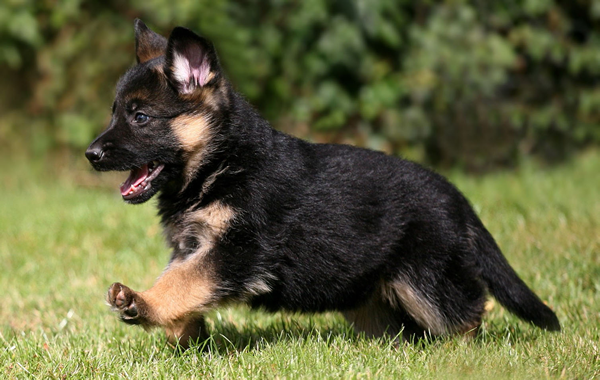
\includegraphics[height=4cm]{mascota.png}\\

Mi otra mascota el el gato de la figura \ref{fig:gato}

\begin{figure}[h] %Entorno para imagenes.
    \centering
    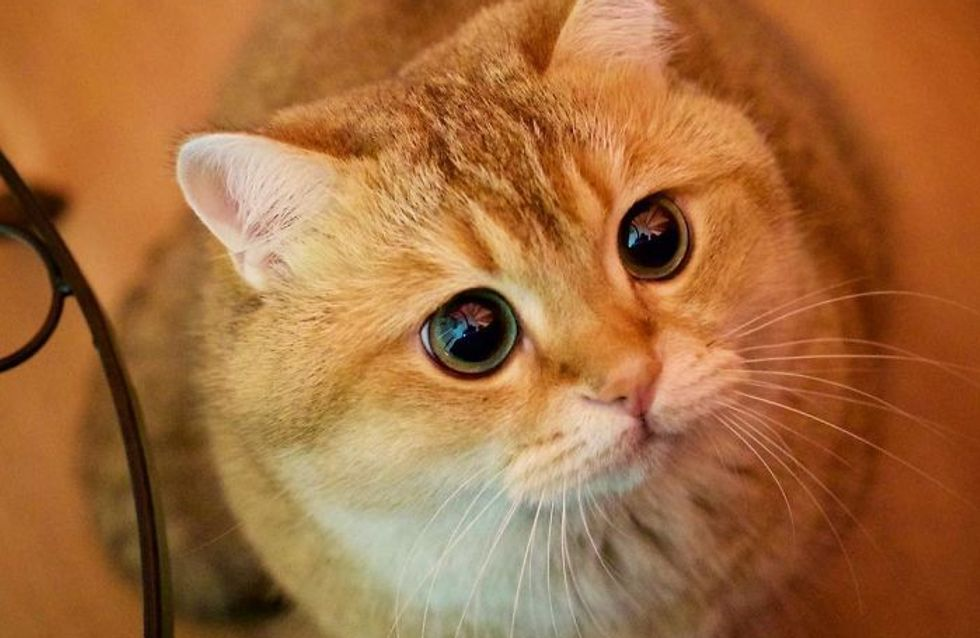
\includegraphics[height=4cm]{gato.jpg}
    \caption{Éste es mi gato.}
    \label{fig:gato}
\end{figure}

%%%%%%%% Listas %%%%%%%%%%%%
Mis mascotas son:\\
\begin{itemize}[noitemsep,nolistsep]  %Lista
    \item gato
    \item perro
    \item hamster
\end{itemize}

Mis deberes son:
\begin{enumerate}[noitemsep,nolistsep]  %Lista enumeradas
    \item Dar de alimientar a las mascotas.
    \item Bañar a las mascotas.
\end{enumerate} 

%%%%%%Ecuaciones%%%%%

\subsection{Mis ecuaciones}

La relación de masa energías es: $E=mc^2$.
Teorema de pitagoras es
\begin{equation} 
    c^2=a^2+b^2
\end{equation}

\section{Texto}
\lipsum[1] %Generación de Texto Aleatorio

\section{tablas}

%%%%%%%% Tablas %%%%%%%%%
\begin{tabular}{||c|c||}
    \hline 
    mascota & edad(Años)\\ \hline \hline
    perro & 3 \\ \hline
    gato & 4\\ \hline
    hamster & 1 \\ \hline
\end{tabular}

\end{document}